% ============================================
% VII. EMPIRICAL PERFORMANCE ANALYSIS
% ============================================
\section{Empirical Performance Analysis}
\label{sec:results}


Table~\ref{tab:performance_summary} and Figures~\ref{fig:throughput}--\ref{fig:block_utilization} summarise results across all five stages, demonstrating systematic progression from a 0.25~tx/sec synchronous baseline to the 31.19~tx/sec proposed architecture.


\begin{table*}[htbp]
    \centering
    \caption{Summary of Performance Metrics Across Architectural Stages}
    \label{tab:performance_summary}
    \resizebox{\textwidth}{!}{%
    \begin{tabular}{cp{3cm}ccccc}
        \toprule
        \textbf{Arch} & \textbf{Key Feature} & \textbf{Throughput} & \textbf{Total Time} & \textbf{Avg Latency} & \textbf{P99 Latency} & \textbf{Avg Tx/Block} \\
        & & (tx/sec) & (s) & (s) & (s) & \\
        \midrule
        1 & Sync, Single-Wallet & 0.25 & 3999.79 & 4.000 & 4.206 & 1.00 \\
        2 & Async, Single-Wallet & 13.22 & 75.67 & 2.916 & 4.913 & 52.63 \\
        3 & Multi-Thread, Async, Single-Wallet & 18.04 & 55.42 & 2.959 & 5.177 & 71.43 \\
        4 & Unsync Multi-Thread, Multi-Wallet & 24.16 & 41.39 & 27.211 & 28.972 & 111.11 \\
        \textbf{5 (Proposed)} & Symbol-Sharded, Lock-Free, Multi-Wallet & \textbf{31.19} & \textbf{32.06} & 15.432 & 30.136 & \textbf{125.00} \\
        \bottomrule
    \end{tabular}%
    }
\end{table*}

\begin{figure}[htbp]
    \centering
    \begin{subfigure}[b]{0.32\textwidth}
        \centering
        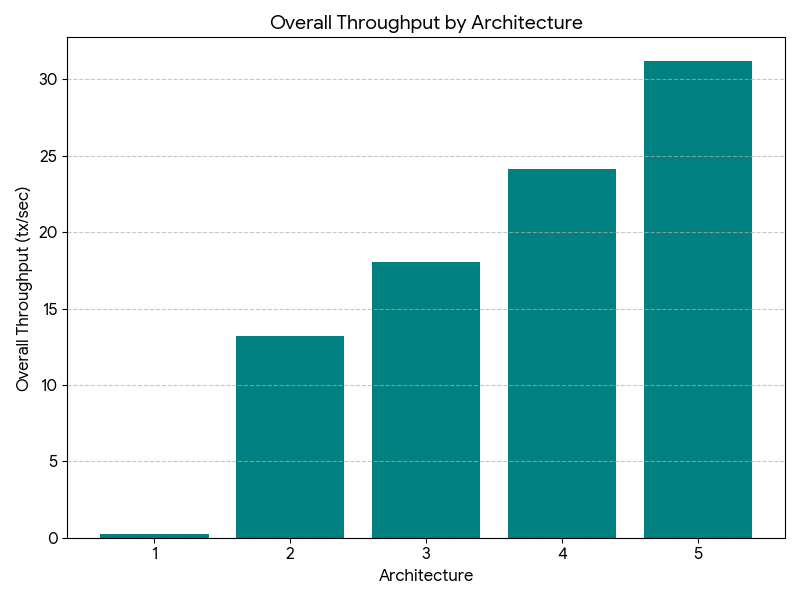
\includegraphics[width=\textwidth]{images/stat1.png}
        \caption{Throughput}
        \label{fig:throughput}
    \end{subfigure}
    \hfill
    \begin{subfigure}[b]{0.32\textwidth}
        \centering
        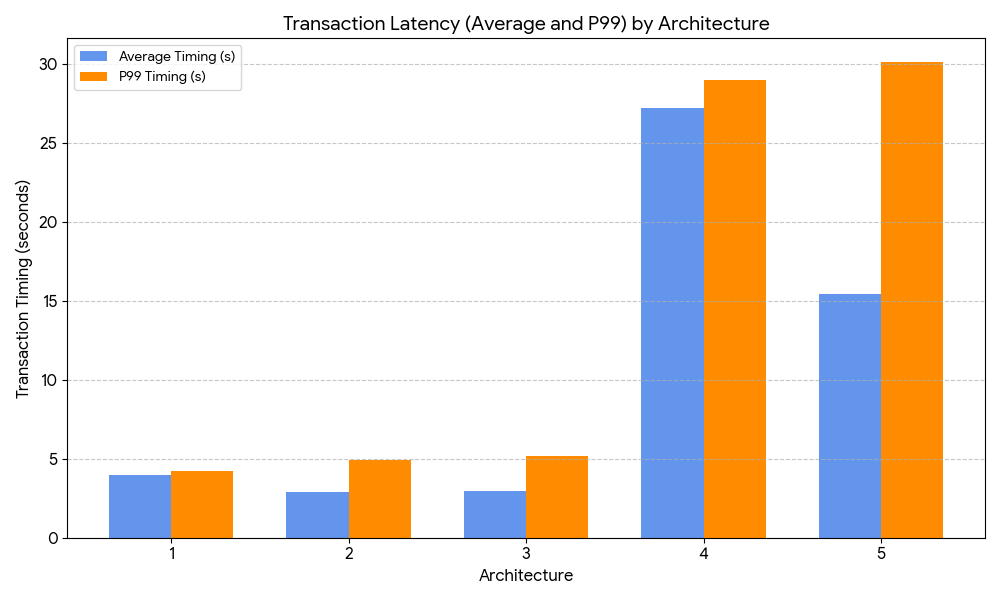
\includegraphics[width=\textwidth]{images/stat2.png}
        \caption{Latency}
        \label{fig:latency}
    \end{subfigure}
    \hfill
    \begin{subfigure}[b]{0.32\textwidth}
        \centering
        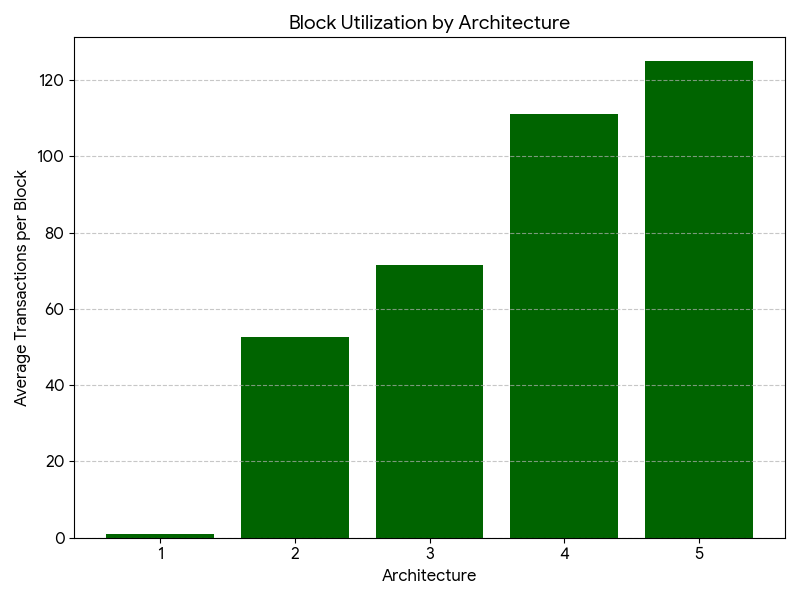
\includegraphics[width=\textwidth]{images/stat3.png}
        \caption{Block Utilization}
        \label{fig:block_utilization}
    \end{subfigure}
    \caption{Performance metrics across architectural stages.}
    \label{fig:performance_metrics}
\end{figure}

\subsection{From Synchronous to Asynchronous: Overcoming Network Latency}

Throughput improved most significantly in the transition from Architecture~1 to Architecture~2. Decoupling submission from synchronous confirmation increased throughput over 50$\times$, from 0.25~tx/sec to 13.22~tx/sec, confirming that the naive implementation was bottlenecked by block time. Average latency dropped from 4.0s to 2.9s as asynchronous submission enabled more efficient transaction batching~\cite{ding2018batching,hennessy2017computer}.

\subsection{The Nonce Bottleneck: The Limits of Single-Wallet Parallelism}

Architecture~3's multi-threaded submission provided a key insight: despite parallel processing, throughput increased only 36\%, from 13.22~tx/sec to 18.04~tx/sec. Because nonce requirements are strictly sequential, threads serialized at the blockchain level, limiting parallelization gains consistent with Amdahl's Law~\cite{amdahl1967validity}. True parallelization requires addressing the single-wallet nonce constraint.

\subsection{Server-Side Contention Emerges}

Architecture~4 introduced a wallet pool to circumvent nonce constraints, increasing throughput to 24.16~tx/sec. However, this came at significant cost: average latency rose sharply from ~3s to over 27s (P99: ~29s). Removing the blockchain-level bottleneck shifted contention to the server~\cite{moir2018concurrent}. Without coordination, threads competed for shared resources, causing cache thrashing and lock convoying; transactions queued locally before reaching the network.

P99 latency (28.97~s) relative to the average (27.21~s) indicates most transactions experienced similar delays, a systemic bottleneck rather than occasional outliers. This pattern is characteristic of lock contention, where threads wait for exclusive access to shared resources.

\subsection{The Proposed Solution: Symbol-Sharding and Lock-Free Queues}

Architecture~5 introduced symbol-sharding and lock-free queues to address server-side contention. This achieved the highest throughput at 31.19~tx/sec (29\% over Architecture~4) while reducing average latency by 43\%, from 27.2s to 15.4s. Partitioning by trading symbol and using CAS-based lock-free queues effectively eliminates server-side resource competition~\cite{harris2001pragmatic}.

P99 latency remained high (~30s), indicating tail latency persists for highly contended symbols that create temporary within-shard backlogs, a challenge for future work.

\subsection{Block Utilization, Burst Handling, and Scalability}

Block utilization rose with throughput improvements: from 1.0~tx/block (baseline) to 125.0~tx/block (Architecture~5). Gas usage remained stable (146,194--152,603 gas/tx), confirming gains were purely architectural.

The observed 125~tx/block exceeds the theoretical maximum of ~71.7~tx/block, demonstrating successful burst handling: the architecture submitted transactions at 1.74$\times$ the blockchain's sustained capacity (~17.93~tx/sec), with excess transactions queuing in the mempool. This is critical for trading workloads where market events trigger sudden order spikes.

The architecture scales linearly with blockchain capacity increases (Layer~2, higher gas limits, faster consensus). Because the submission layer sustains rates exceeding blockchain capacity, symbol-sharded pipelines operate independently with negligible overhead. The submission layer is demonstrably not the bottleneck.

\subsection{Answering the Research Questions}

Our empirical results provide clear answers to each of the research questions posed in the introduction.

\textbf{Answer to RQ1 (Throughput Ceiling and Shifting Bottlenecks):} The throughput ceiling is \textbf{31.19~tx/sec}, a \textbf{2.8$\times$ improvement} over conventional asynchronous multi-threaded designs. The ablation reveals bottlenecks \textit{shifting}: synchronous I/O (Arch~1$\rightarrow$2) $\rightarrow$ nonce serialization (Arch~2$\rightarrow$3) $\rightarrow$ server-side contention (Arch~3$\rightarrow$4) $\rightarrow$ submission layer no longer limiting (Arch~5). This demonstrates \textbf{contributions C3 and C4}.

\textbf{Answer to RQ2 (Adapting HFT Patterns to Blockchain):} Lock-free HFT patterns adapt successfully to blockchain submission with careful nonce co-design. Symbol-sharded, CAS-based queues eliminate server-side contention, though persistent high P99 latency (~30s) indicates within-shard contention for popular symbols remains a challenge (\textbf{contribution C1}).

\textbf{Answer to RQ3 (Architectural Design vs. Latency):} Architectural design significantly impacts settlement latency. The 9$\times$ latency increase from Architecture~3 (2.96s) to Architecture~4 (27.21s) resulted solely from server-side contention (\textbf{contribution C5}). The symbol-sharded design reduced latency by 44\% while increasing throughput, demonstrating that both metrics can improve concurrently.

% References for this section are in the main bibliography

